\documentclass[border=10pt]{standalone}

\usepackage{tikz}
\usepackage{tikzsymbols}
\usetikzlibrary{calc,patterns,shapes.geometric}

\def\centerarc[#1](#2)(#3:#4:#5){\draw[#1] ($(#2)+({#5*cos(#3)},{#5*sin(#3)})$) arc (#3:#4:#5);}

\begin{document}
	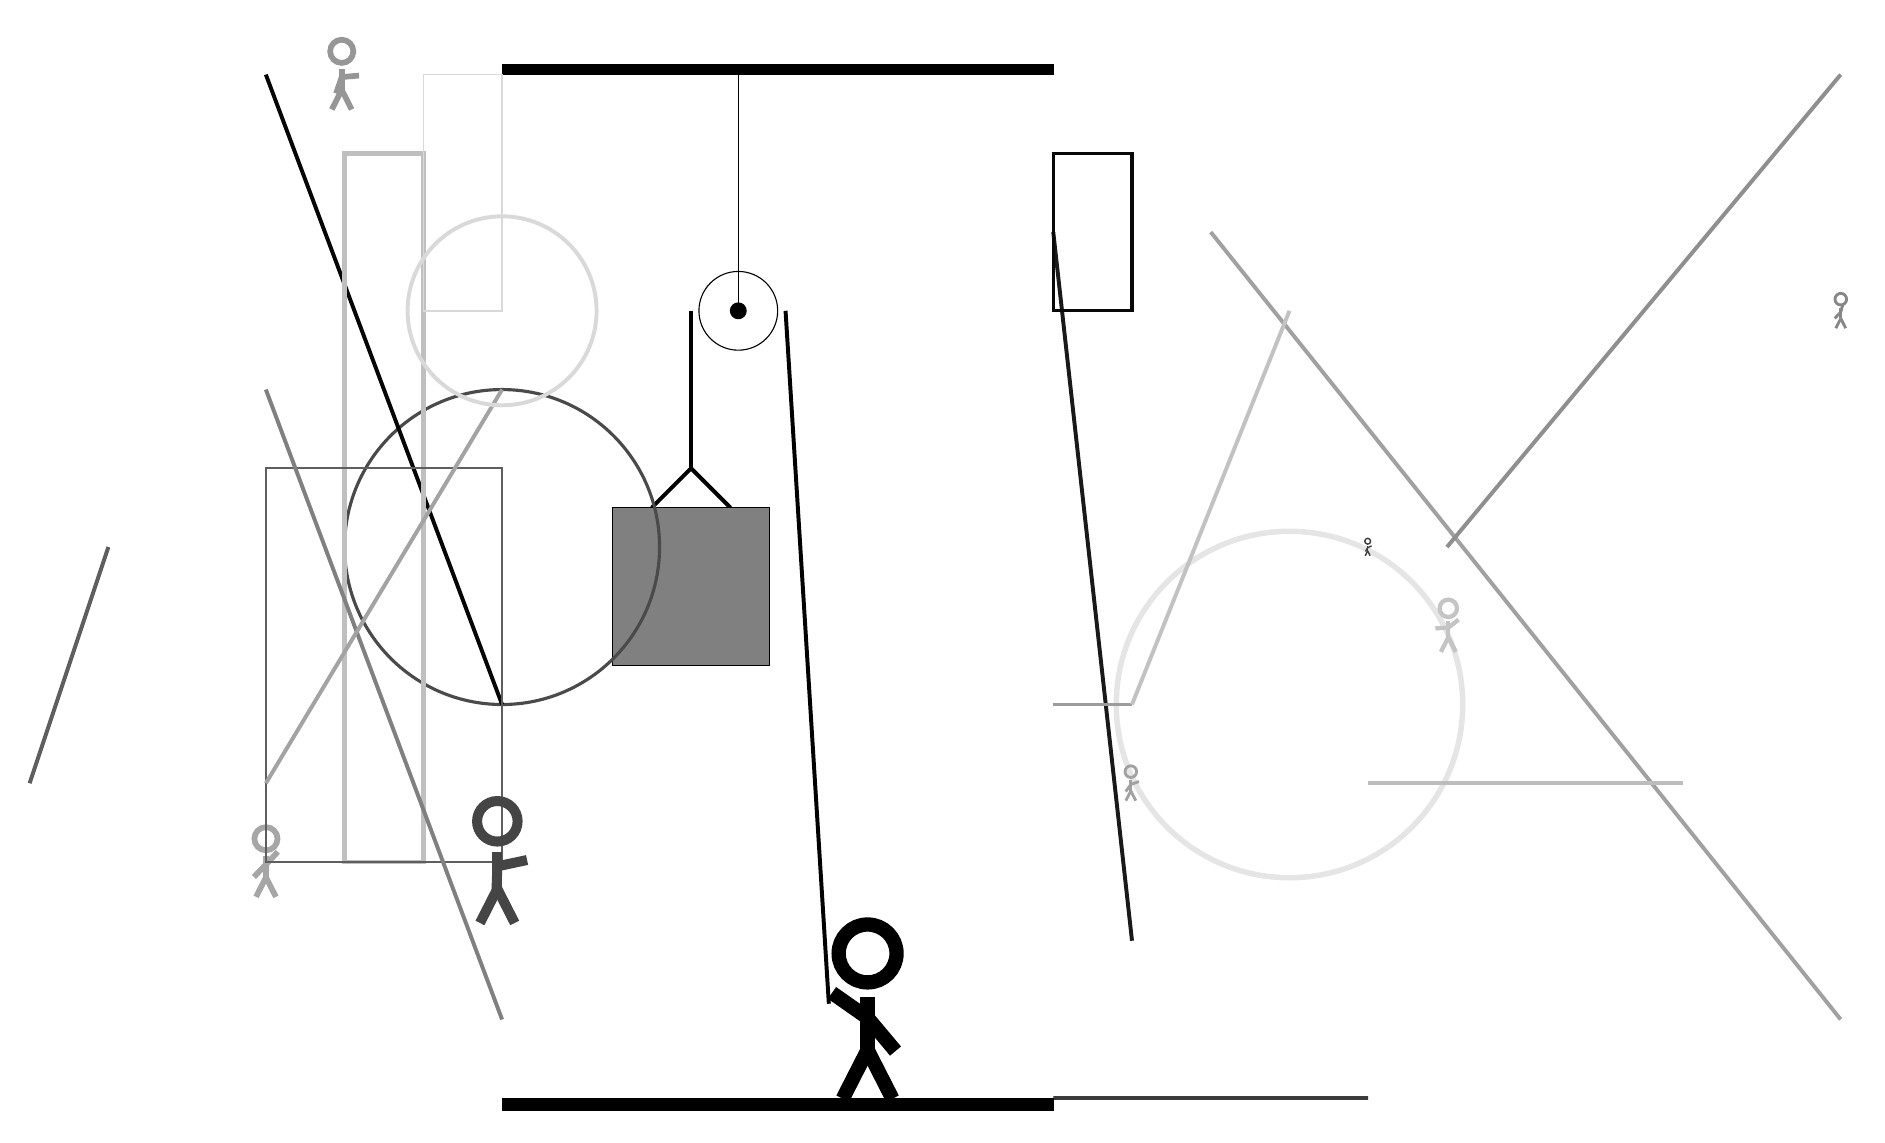
\begin{tikzpicture}
		%%%%% START %%%%%
		
		\draw[fill=black] (-2, 10) rectangle (5, 10.125);
		
		\draw (1, 7) circle (0.5);
		\draw[fill=black] (1, 7) circle (0.1);
		\draw (1, 10) -- (1, 7);
		
		\draw[line width=0.5mm] (-0.1, 4.5) -- (0.4, 5.0) -- (0.9, 4.5);
		\draw[fill=black!50] (-0.6, 4.5) rectangle (1.4, 2.5);
		
		\draw[line width=0.5mm] (0.4, 7) -- (0.4, 5.0);
		\centerarc[line width=0.5mm](1, 7)(0:180:0.6);
		\draw[line width=0.5mm](1.6, 7) -- (2.15, -1.8);
		
		\node at (2.6, -1.9) {\Strichmaxerl[10][-35][-50]};
		
		\draw [line width=0.7mm, color=black!10](8, 2) circle (2.2);
		
		\draw[line width=0.5mm, color=black!90](6, -1) -- (5, 8);
		\draw[line width=0.5mm, color=black!77] (5, -3) rectangle (9, -3);
		\draw[line width=0.5mm, color=black!37](7, 8) -- (15, -2);
		\node[line width=0.5mm, color=black!35] at (-5, 0) {\Strichmaxerl[4][46][47]};
		
		\draw [line width=0.4mm, color=black!71](-2, 4) circle (2.0);
		
		\draw[line width=0.5mm, color=black!26](9, 1) -- (13, 1);
		\draw[line width=0.5mm, color=black!98](-2, 2) -- (-5, 10);
		\draw[line width=0.6mm, color=black!25] (-3, 0) rectangle (-4, 9);
		\draw[line width=0.3mm, color=black!63] (-2, 5) rectangle (-5, 0);
		
		\draw[line width=0.5mm, color=black!50](-5, 6) -- (-2, -2);
		\node[line width=0.4mm, color=black!37] at (6, 1) {\Strichmaxerl[2][54][20]};
		\draw[line width=0.5mm, color=black!39](5, 2) -- (6, 2);
		\node[line width=0.4mm, color=black!73] at (-2, 0) {\Strichmaxerl[7][88][12]};
		\draw[line width=0.5mm, color=black!24](6, 2) -- (8, 7);
		\node[line width=0.6mm, color=black!47] at (15, 7) {\Strichmaxerl[2][46][75]};
		\node[line width=0.4mm, color=black!76] at (9, 4) {\Strichmaxerl[1][60][24]};
		\draw[line width=0.2mm, color=black!15] (-3, 7) rectangle (-2, 10);
		\node[line width=0.7mm, color=black!41] at (-4, 10) {\Strichmaxerl[4][71][5]};
		\draw[line width=0.5mm, color=black!63](-7, 4) -- (-8, 1);
		\draw[line width=0.5mm, color=black!36](-5, 1) -- (-2, 6);
		\node[line width=0.6mm, color=black!23] at (10, 3) {\Strichmaxerl[3][3][38]};
		\draw [line width=0.5mm, color=black!15](-2, 7) circle (1.2);
		\draw[line width=0.4mm, color=black!97] (6, 9) rectangle (5, 7);
		\draw[line width=0.5mm, color=black!44](10, 4) -- (15, 10);
		
		
		\draw[fill=black] (-2, -3) rectangle (5, -3.15);
		
		%%%%% END %%%%%
	\end{tikzpicture}
\end{document}